\section{Tribler}

Tribler is an application that enables its users to find, consume and share content through a peer-to-peer (P2P) network. The application is currently available for Windows, Mac and Linux. Tribler facilitates finding and sharing content in a fully decentralized manner so that no central server is needed. Furthermore, to tackle the issue of people who only download(leech) content, Tribler makes use of a reputation system which encourages users to actively participate in uploading (seeding) content. Tribler also includes a VoD service which allows users to first search any video and then click on play so that the video will be streamed to the user.

\begin{figure}[h]
	\centering
	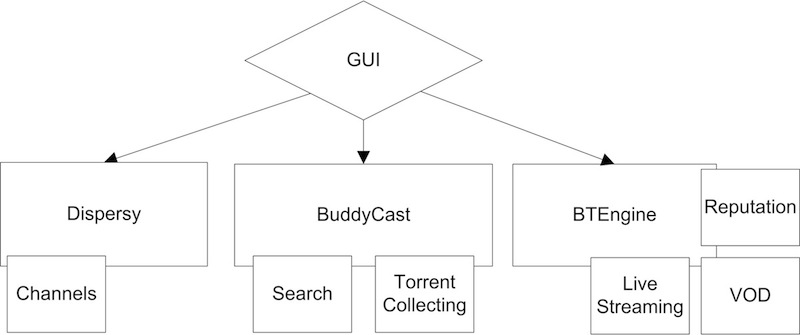
\includegraphics[scale=0.4]{vod/images/tribler_component_overview.jpg}
	\caption{The architecture of Tribler\protect\footnotemark}
	\label{fig:tribler_components}
\end{figure}
\footnotetext{http://sigmm.org/records/records1201/featured03.html}
\noindent Tribler consists out of four major components as can also be seen in figure \ref{fig:tribler_components}:
\begin{itemize}
	\item GUI: the graphical user interface.
	\item BTengine: An implementation of the BitTorrent\footnote{http://www.bittorrent.com/} protocol.
	\item BuddyCast: a protocol used to find peers with the same taste as the user\cite{tribler}
	\item Dispersy: a fully decentralized system for data bundle synchronization\cite{dispersy}.
\end{itemize}

\subsection{BTengine}
BitTorrent is a protocol which allows for P2P file sharing. The protocol allows users to join a swarm of hosts to download and upload files. For a user to share a file it can create a torrent descriptor file which contains information about the file. The torrent can then be distributed over the Internet via e-mail, a link on a website, etc. Other users with the torrent can connect to this host, called a seeder, and ask for pieces of this file. After all pieces are collected, the leecher becomes a seeder and other leechers can download from the new seeder. This way, the files are distributed over the Internet without needing any central server.\\ 
The BTengine in Tribler includes a reputation system, where the user is rated for their upload to download ratio. This helps to minimize the effects of free riding, where users only download, because the user with a low ratio will be given lower speed peers to connect to. As said earlier, the BTengine (As of Tribler version 6.1) uses an implementation of BitTorrent called: Libtorrent.

\subsubsection{Libtorrent}
Libtorrent is a C++ implementation of BitTorrent for embedded devices as well as desktops\footnote{http://www.rasterbar.com/products/libtorrent/}.The interface is well documented and is designed to be CPU- and memory-efficient as well as easy to use.

\subsubsection{Libswift}
The libswift protocol is designed to operate at the transport layer, it is designed to be very lightweight, have non-intrusive congestion control and automatic disk space management.\footnote{http://libswift.org/} It is developed by the PDS department as part of the P2P-Next project\footnote{http://p2p-next.org/}.

\subsection{BuddyCast}
The BuddyCast protocol is used to find peers with similar taste, so Tribler can give recommendations to what the user might like and thus discover new content. 

\subsection{Dispersy}
Dispersy is used to spread data bundles over the Internet in a fully decentralized way. This could potentially remove the need for central servers for services as Facebook or Wikipedia. In Tribler it is used for creating the channels. Each channel has different torrents bundled together to form a sort of playlist about one topic such a single genre or the new 2013 releases. This makes the discovery of new files that the user might like, easier for the user.

\subsection{GUI}
\begin{figure}[h]
	\centering
	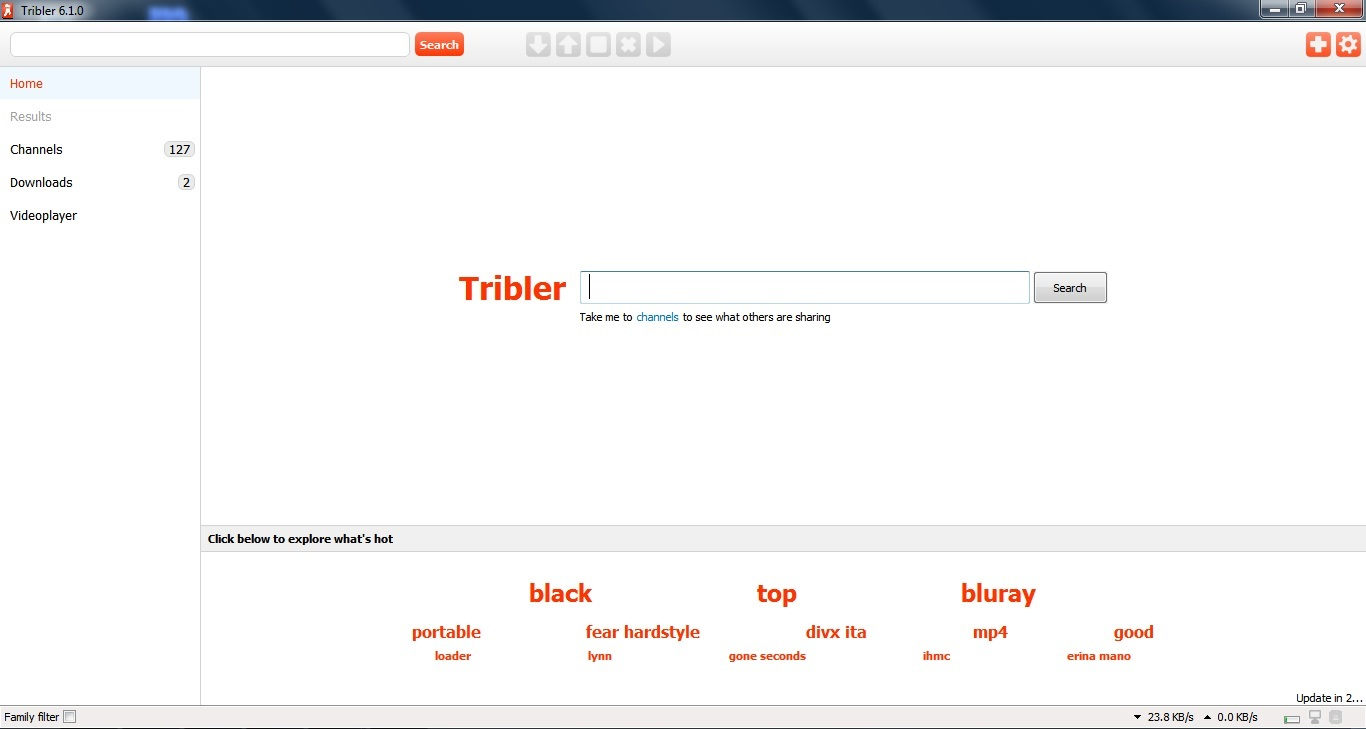
\includegraphics[scale=0.35]{vod/images/tribler_gui.jpg}
	\caption{Tribler's GUI}
\end{figure}
The GUI has a number of elements to it, resembling Tribler's main features:
 \begin{itemize}
	\item Top bar\\ This includes a search bar, a number of controls, and buttons to go into the settings and download external torrents. The controls include a button to start streaming the video instead of having to wait for it to be completely downloaded.
	\item Left pane\\ The left pane gives an overview of the different pages to visit. Channels is a page where collections of content are bundled so the user can browse through them. The page below, the downloads page, shows which torrents have been downloaded and what the status is of the current download. The next page is the videoplayer where videos can be watched and streamed.
	\item Bottom bar\\ At the bottom, information can be found how fast the download is going, as well as the upload and more information about how much peers the user is connected to.
\end{itemize}

